\documentclass{article}
\usepackage{neurips_2026}
\usepackage[utf8]{inputenc}
\usepackage[T1]{fontenc}
\usepackage{hyperref}
\usepackage{url}
\usepackage{booktabs}
\usepackage{amsfonts,amsmath,amssymb}
\usepackage{graphicx}

\title{The Asymmetry Principle: A Region-Anchored, Citation-Audited Index of Frontier AI Risk Across Africa}

\author{Anonymous Authors\\Africa in AI @ NeurIPS 2026 (double-blind submission)}

\begin{document}
\maketitle

\begin{abstract}
Frontier AI risk on the African continent does not present as a scaled-down version of the profile
modeled in the United States, European Union, or China. A field study of 57 interviews with 27 former
members of Boko Haram reports use of consumer frontier AI by an armed group in northeast Nigeria
(Juelich, 2026); because that evidence is self-reported and not forensically corroborated in public, we
treat it as a credible but untriangulated account. TransUnion Africa reports a roughly 1{,}200\%
year-over-year rise in deepfake incidents in South Africa, concentrated in banking and fintech.
Kenya's 2022 electoral information environment saw over 550{,}000 posts screened for toxicity by AI
classifiers. We study four anchor states (Egypt, Nigeria, Kenya, South Africa) standing in for North,
West, East, and Southern Africa, and add a short unscored section on the Central African mineral supply
chain beneath global compute. We build a four-component index (AFAIRI): internet exposure (E), reported
scam victimization from one harmonized four-country survey (H), a governance deficit that scores
enforcement capacity and not only legislative existence (G), and infrastructure disruption from grid
failures and subsea-cable outages (I). A Monte Carlo analysis over index weights and independent input
error finds \emph{no} robustly top-ranked state: South Africa has the highest mean and ranks first in
about 47\% of sampled weightings, Egypt in 31\%, Nigeria in 15\%, Kenya in 7\%, and no state outscores
another on every component. An earlier claim that Southern Africa's top ranking is robust (90--95\%) did
not survive a construct revision and is withdrawn. Every quantitative claim traces to a cited source, and
an appendix logs the corrections made in review, including figures that were fabricated in an earlier
draft and removed. We close with a governance architecture scoped to what the regional evidence supports.
\end{abstract}

\section{Introduction: the Asymmetry Principle}
Frontier AI safety frameworks built in the United States, European Union, and China assume infrastructure
that is not uniform across Africa: stable power grids, formal banking clearinghouses, biological-material
screening, and mature statutory enforcement (Anthropic, 2024; European Union, 2024). Where that baseline
holds, frontier AI risk is modeled around misalignment, intellectual-property infringement, and
long-horizon loss of control. Large parts of the continent instead combine rapid consumer AI adoption with
material gaps in that baseline. We call this the \textbf{Asymmetry Principle}: the same model capability
produces different realized failure modes depending on the infrastructural density and governance capacity
of the environment into which it is deployed. This is a qualitative organizing claim, not a fitted
function; no panel dataset spanning enough countries and years exists to estimate one, and we do not claim
to have built one.

\paragraph{Design.} Each region is represented by one anchor state. This is a case-study design, not a
regional average, and results should not be read as describing every state in a region. Region stays a
useful unit because several phenomena cross borders: Boko Haram's integration into Islamic State networks
connects to a jihadist ecosystem that includes Al-Shabaab in East Africa; West African cyber-fraud actors
operate cells across the continent, including in South Africa; and pre-existing governance-capacity gaps now
interact with AI-enabled tooling. Central Africa is not scored (Section~\ref{sec:limits}) but is not ignored:
Section~\ref{sec:supply} addresses the Democratic Republic of Congo's role as the dominant source of mined
cobalt, the physical supply-chain dimension of the same asymmetry.

\paragraph{Five claims.} The paper is organized around five claims, each tied to specific evidence.
\textbf{C1 (framing).} The Asymmetry Principle: the same frontier-AI capability produces different realized
failure modes across environments, and the four anchor states instantiate four distinct modes rather than one
scaled to different sizes. \textbf{C2 (headline result).} Under a construct-valid, weight-agnostic Monte Carlo,
\emph{no} African anchor state is robustly the highest-risk: no ordering holds across the weight simplex, and
no state dominates another on every component (Section~\ref{sec:index}). \textbf{C3 (methodological).} Composite
frontier-risk rankings are dominated by construct choice, not data: replacing environmental and inclusion
proxies with measures of reported victimization, enforcement, and disruption overturns the earlier draft's
``Southern Africa robust at 90--95\%'' and drops South Africa's ranked-first share below 50\%. \textbf{C4
(evidence integrity).} Under systematic triangulation, the strongest \emph{corroborated} evidence of African
frontier-AI misuse is fraud, not terrorism: Nigeria-origin AI-assisted scam networks are platform-corroborated
(OpenAI, 2025), whereas the widely cited insurgent-AI account is self-reported and untriangulated. \textbf{C5
(governance).} Enforcement, not legislation, is the binding governance gap: scoring enforcement capacity
separately from statute reveals that a state with a published AI strategy (Egypt) can carry the largest
enforcement gap while the weakest strategy status (Nigeria) coexists with the strongest penalty record. We also
release a citation-and-methodology audit log that documents, rather than hides, what earlier drafts got wrong,
including figures that were fabricated and removed.

\section{Four anchor states}
\textbf{North Africa (Egypt).} Strong laboratory biosafety practice assessed through the WHO Joint External
Evaluation, alongside the largest governance-enforcement gap in the set: its data-protection regime begins
enforcement only in October 2026. Egypt also ran national load-shedding for roughly 202 days in 2024.
\textbf{West Africa (Nigeria).} The self-reported insurgent-misuse account (Juelich, 2026) and the most
severe measured infrastructure disruption (12 national grid collapses in 2024), coupled with, on a
penalty-issuance proxy, the strongest data-protection enforcement record (a USD 32.8M action against Meta).
\textbf{East Africa (Kenya).} A mobile-first ecosystem, the highest reported scam victimization of the four
states, electoral information-integrity strain in 2022, and repeated 2024 blackouts.
\textbf{Southern Africa (South Africa).} A roughly 1{,}200\% year-over-year rise in deepfake incidents
concentrated in banking and fintech (TransUnion Africa, 2025), the highest internet exposure, and the
highest mean index score.

\section{The AFAIRI composite index}
\label{sec:index}
AFAIRI is a composite proxy index in the family of the Human Development Index or ND-GAIN: a few individually
cited indicators combined under a disclosed weighting scheme. It is \emph{not} validated against an external
ground truth of realized AI-enabled harm, because no such dataset exists across these states. It is a
structured comparison of four documented case studies, not a risk-prediction model.

\paragraph{Specification.} $\mathrm{AFAIRI}(s) = w_E E + w_H H + w_G G + w_I I$ with
$w_E+w_H+w_G+w_I=1$. \emph{Exposure} $E$ is 2023 internet penetration (World Bank WDI, untransformed).
\emph{Reported scam victimization} $H$ is the share of adults reporting a scam in the previous 12 months,
from the Global Anti-Scam Alliance's \emph{State of Scams in Africa 2025}, a survey of 4{,}000 adults
covering exactly these four states. \emph{Governance deficit} $G = 100-(A+B+C)$ scores AI-strategy status
($A$), AI-specificity of cybercrime law ($B$), and enforcement capacity ($C$, keyed to whether the
data-protection authority has issued monetary penalties and of what size). \emph{Infrastructure disruption}
$I$ sums a grid-failure tier and a subsea-cable-outage score for calendar year 2024. Every threshold (for
example USD 1M, 90 days, six collapses) was fixed before the scores were computed. Full rubrics, source
values, and per-criterion limitations are in the manuscript; Table~\ref{tab:components} gives the resulting
component matrix.

\begin{table}[t]
\centering\small
\caption{AFAIRI v4 component matrix (0--100 scale). See Figure~\ref{fig:components}.}
\label{tab:components}
\begin{tabular}{lcccc}
\toprule
Anchor state (region) & $E$ exposure & $H$ victimization & $G$ gov.\ deficit & $I$ disruption \\
\midrule
Egypt (North) & 74.0 & 39.0 & 62.5 & 50.0 \\
Nigeria (West) & 40.1 & 73.0 & 12.5 & 75.0 \\
Kenya (East) & 32.1 & 83.0 & 37.5 & 50.0 \\
South Africa (Southern) & 78.3 & 77.0 & 37.5 & 50.0 \\
\bottomrule
\end{tabular}
\end{table}

\begin{figure}[t]
\centering
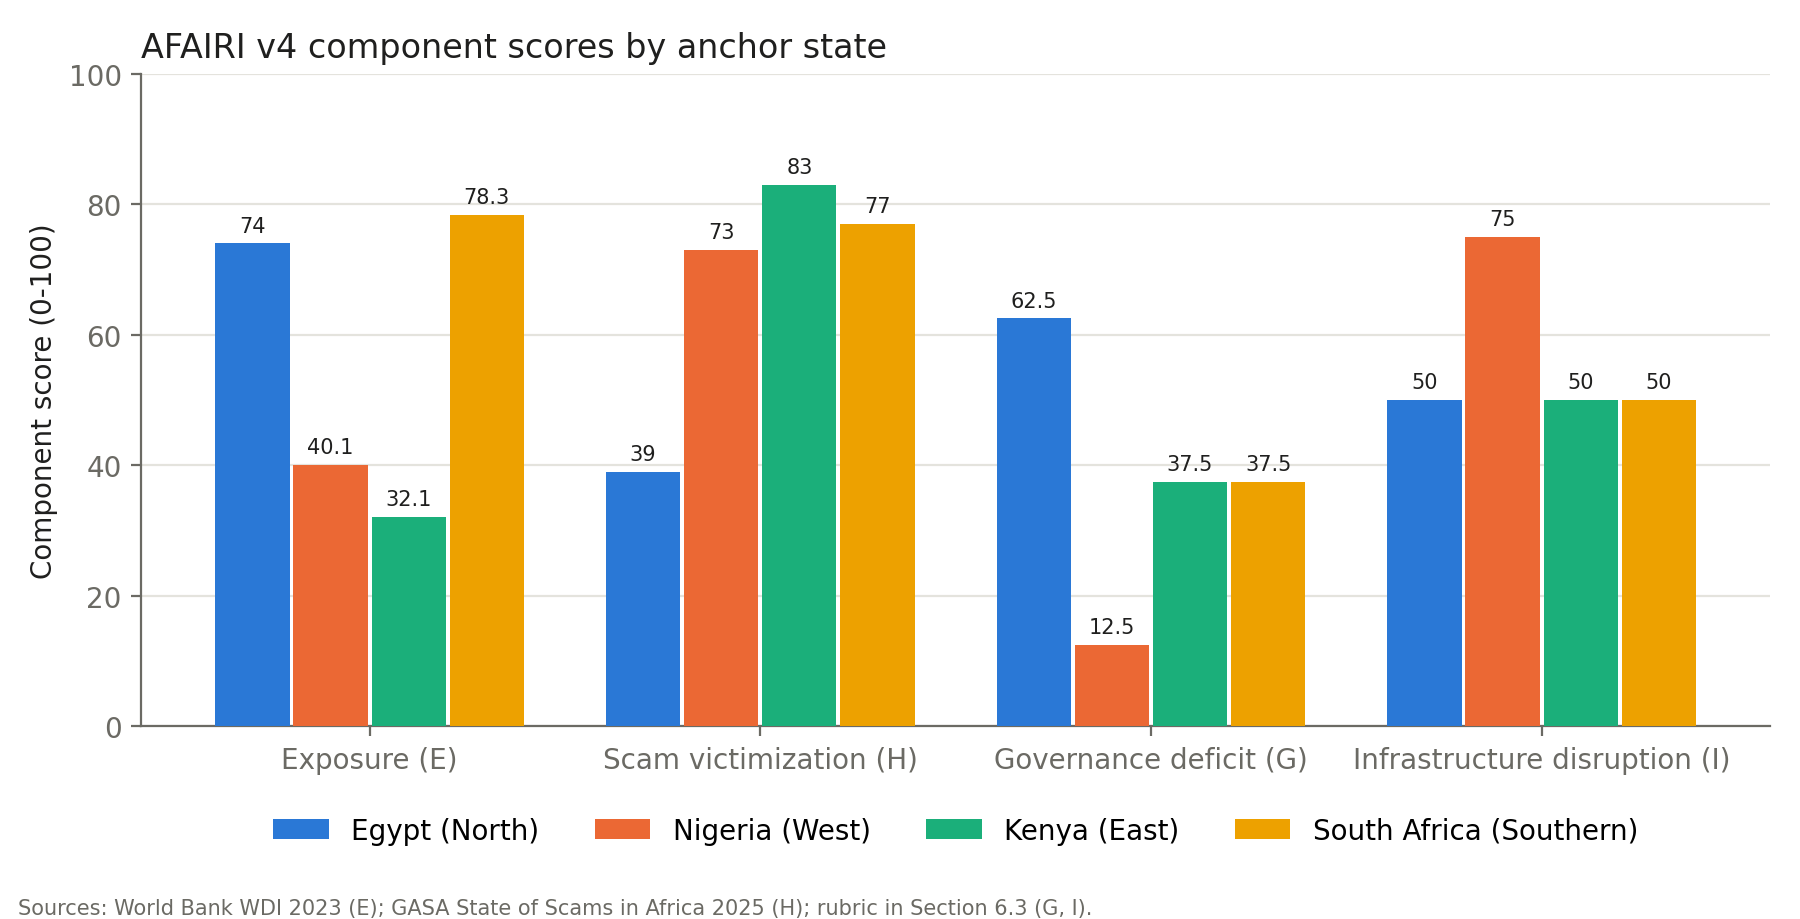
\includegraphics[width=0.66\linewidth]{figures/fig1_components.png}
\caption{AFAIRI v4 component scores by anchor state ($E$, $H$, $G$, $I$; 0--100), values printed on each
bar. Data as in Table~\ref{tab:components}.}
\label{fig:components}
\end{figure}

\paragraph{Sensitivity analysis.} We drew $N=10^4$ weight vectors from a symmetric Dirichlet$(1,1,1,1)$
(uniform over the weight simplex), recomputed AFAIRI for each state, and repeated with independent
multiplicative perturbations of each of the 16 inputs at $\pm10\%$ and $\pm25\%$, and with a coupling term
restored as a robustness run (seed 42). ``Share ranked first'' is the fraction of the sampled weight space in
which a state scores highest; it is \emph{not} the probability that a state is in fact the riskiest, because
the uniform prior over weights is itself a modeling choice. Reported ranges are 2.5th--97.5th percentiles of
the score across weightings: sensitivity ranges, not confidence intervals.

\begin{table}[t]
\centering\small
\caption{Weight-only sensitivity ($N=10^4$ Dirichlet draws). No robustly top-ranked state.}
\label{tab:sensitivity}
\begin{tabular}{lccc}
\toprule
State & mean & range (2.5--97.5\%) & ranked first \\
\midrule
South Africa & 60.8 & 45.3--74.5 & \textbf{47.1\%} \\
Egypt & 56.4 & 45.0--67.7 & 31.0\% \\
Nigeria & 50.2 & 25.8--69.6 & 15.2\% \\
Kenya & 50.6 & 37.2--70.8 & 6.7\% \\
\bottomrule
\end{tabular}
\end{table}

\begin{figure}[t]
\centering
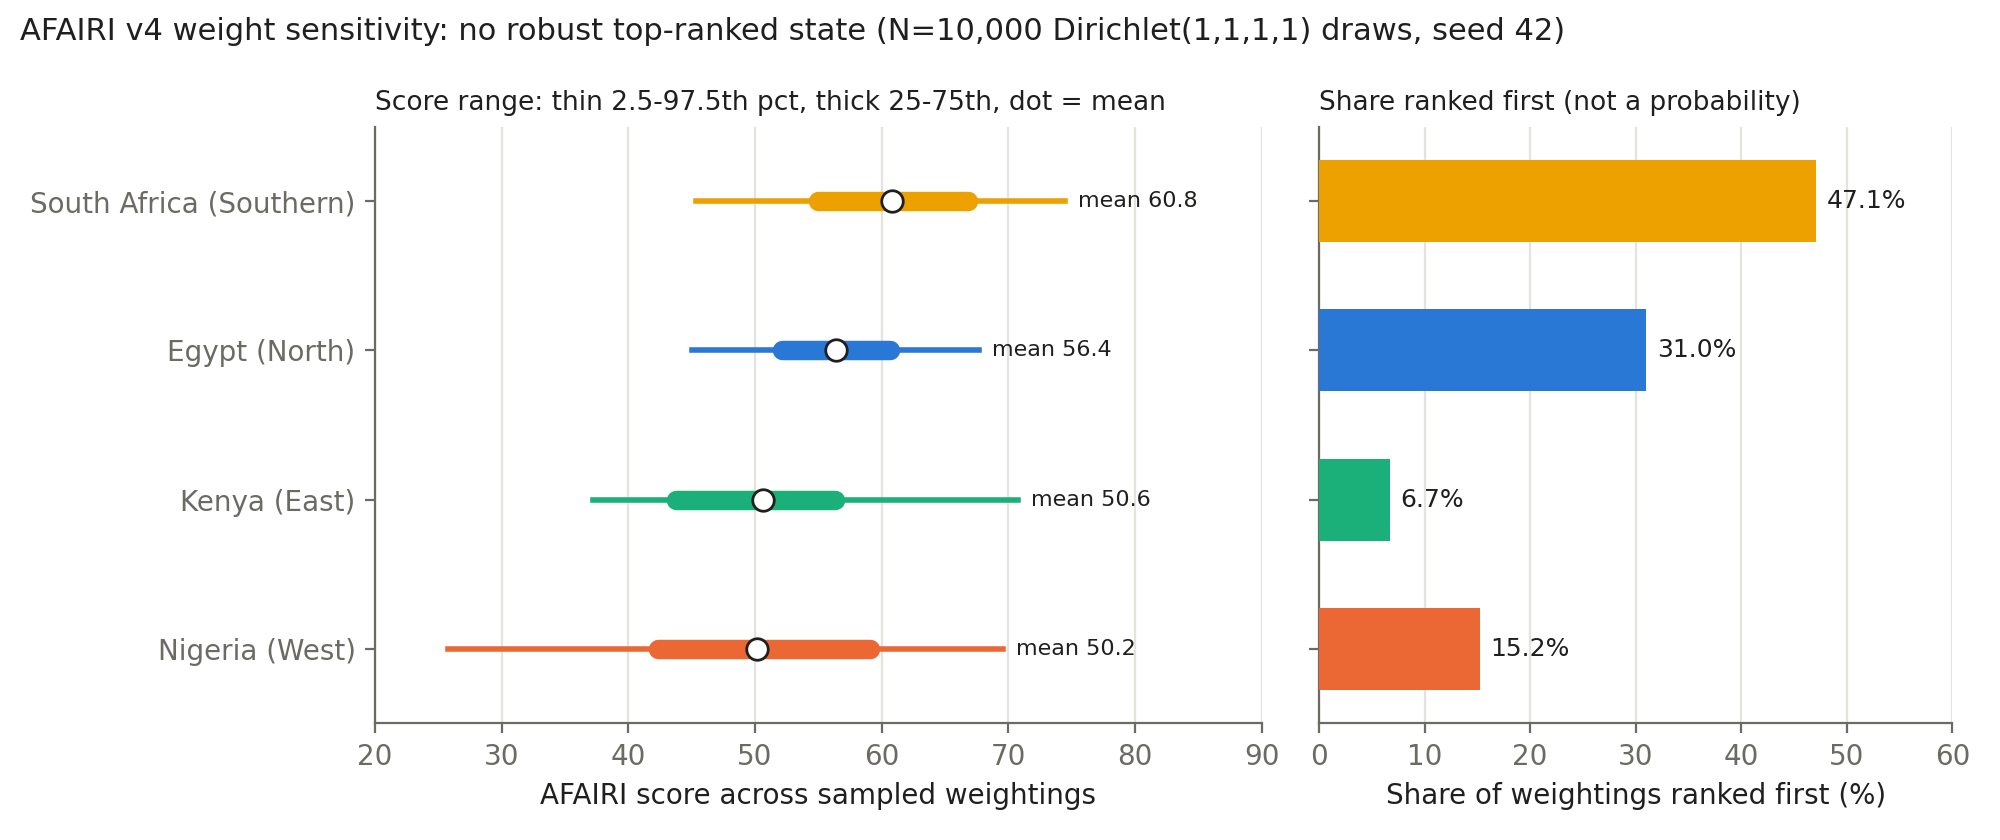
\includegraphics[width=0.9\linewidth]{figures/fig2_sensitivity.png}
\caption{Weight sensitivity ($N=10^4$ Dirichlet$(1,1,1,1)$ draws, seed 42). Left: distribution of each
state's score across weightings (thin line 2.5--97.5\%, thick line 25--75\%, dot mean). Right: share of
weightings in which each state ranks first. Sensitivity summaries, not confidence intervals or
probabilities.}
\label{fig:sensitivity}
\end{figure}

\paragraph{What the index supports.} South Africa has the highest mean, ranks first most often, and outscores
each other state in a majority of weightings (66\% vs.\ Egypt, 83\% vs.\ Nigeria, 87\% vs.\ Kenya). The
result is stable under input error and the coupling run (Table~\ref{tab:sensitivity}; ranked-first shares move
by at most a few points). What is \emph{not} supported is a claim that any state is robustly highest-risk:
South Africa ranks first in fewer than half of weightings and Egypt in almost a third, because the two are
high on different components (South Africa on victimization, Egypt on governance deficit), and the Kenya--Nigeria
ordering is effectively a coin flip. The earlier ``Southern Africa robust at 90--95\%'' headline came from
constructs that external review found invalid and is withdrawn.

\paragraph{Verification.} A separate script recomputed every component by hand from the rubric (all matched);
confirmed that each state's Dirichlet mean equals the simple average of its four components (matched to within
0.07 on a fresh 200{,}000-draw simulation); and recomputed the ranked-first shares exactly on a
$\approx$176{,}000-point grid over the simplex (South Africa 46.2\%, Egypt 31.1\%, Nigeria 15.3\%, Kenya
7.3\%), agreeing with the random sampling to within one point. Re-running the previous draft's code is how a
jitter implementation error (a single random factor applied to all four components, rather than independent
perturbation) was found and fixed.

\section{Threat-actor characterization}
We label each actor by an evidence tier rather than asserting uniform confidence. The earlier label
``PRIMARY-VERIFIED'' for the Boko Haram study conflated reading a source with verifying its claims and is
retired. \textbf{Boko Haram / ISWAP} (West Africa): reported use of ChatGPT, Claude, Gemini, Grok, Meta AI, and
DeepSeek for tactical planning, explosives, weapons servicing, and operational security, with unlinkable
accounts and pretextual framing to defeat content restrictions (Juelich, 2026). Tier:
\emph{primary-read, self-reported, untriangulated}; a May 2026 seizure of 400+ Starlink terminals corroborates
connectivity but not AI use, and no seized-device forensics or platform disclosure attributing activity to these
groups was located. \textbf{Al-Shabaab} (East Africa): AI-assisted propaganda translation, attributed to a 2025
UN monitoring-team report via secondary coverage (\emph{secondary-corroborated}; the primary UN document was not
read). \textbf{``Yahoo Boys'' / ``AI Boys''} (West Africa, global targets): AI-generated image, voice, and message
content for fraud; \emph{platform-corroborated} at the level of Nigeria-origin AI-assisted scam networks, via
OpenAI's October 2025 threat-intelligence disclosure. \textbf{Black Axe} (transnational): a structured syndicate
with law-enforcement-confirmed fraud (INTERPOL Operation Jackal III; Europol arrests) but \emph{no} confirmed
Black Axe-specific AI use, and none is claimed. Threat-actor activity is deliberately \emph{not} an index input.

\section{Governance architecture and the compute supply chain}
\label{sec:supply}
Each pillar is scoped to its evidence. \textbf{Pillar 1: AU-level red-teaming and evaluation capacity},
motivated by the self-reported workaround pattern (unlinkable accounts, pretextual framing), which is cheap to
add to evaluation suites whether or not the interview claims of uplift hold, plus a forensic-corroboration
workstream so future threat claims can be checked against account and device evidence. \textbf{Pillar 2:
additionality and base-load isolation for new compute}, an environmental-governance recommendation kept
separate from the safety-risk index. \textbf{Pillar 3: application-layer provenance with funded enforcement},
motivated by South Africa's deepfake and digital-banking fraud and platform-corroborated Nigeria-origin fraud:
a C2PA-style provenance standard is only as effective as the authority enforcing it, so Pillar 3 pairs
provenance rules with funded data- and consumer-protection enforcement and algorithmic recourse for victims.

\paragraph{The unscored supply chain.} The asymmetry also runs through the physical supply chain beneath
compute. The DRC accounted for about 74\% of world mined cobalt in 2023, most of it from Chinese-owned or
-controlled operations (USGS, 2024). Cobalt is used in the lithium-ion backup and UPS systems that data centers
and telecom towers depend on. The states whose infrastructure resilience we score therefore depend, like the
rest of the world, on a mineral supply chain concentrated in a Central African state whose governance and
conflict conditions fall outside the index. We flag this as priority future work rather than fill it with
unverified figures.

\section{Limitations}
\label{sec:limits}
Four anchor states stand in for four regions; results do not generalize to every state in a region, and Central
Africa is only discussed qualitatively. $H$ relies on one industry-alliance survey whose country figures were
taken from its public summary and independent coverage, not the members-only full report, and it disagrees with
national loss statistics on South Africa's relative position. Governance and infrastructure thresholds are
author-chosen, not empirically derived. Penalty issuance is an imperfect proxy for enforcement capacity;
oversight budgets were not available in comparable form. Section~4's Boko Haram evidence rests on self-report and
remains untriangulated, and the Al-Shabaab claim rests on secondary reporting of an unread UN document. The
Egyptian biosecurity JEE dates from 2018. Above all, AFAIRI is not validated against realized AI-enabled harm;
an earlier pilot correlating index scores with a labeled harm-event set in this project's repository was
underpowered and found no significant association.

\section{Conclusion}
The four anchor states show structurally different ways in which frontier AI capability meets variable
infrastructure and enforcement capacity: self-reported insurgent misuse and severe disruption in Nigeria,
measured digital-fraud harm in South Africa, electoral information strain and repeated grid failures in Kenya,
and an enforcement gap in Egypt alongside strong laboratory biosafety practice. Revising the index in response
to review changed its headline: once environmental and inclusion proxies are replaced with measures of reported
victimization, disruption, and enforcement, South Africa remains the most frequently top-ranked state but not a
robust one, and Egypt's unenforced data-protection regime makes it a close second. That is a less striking
conclusion than an earlier draft's, and a more defensible one. Grounding African AI-risk analysis in cited,
regionally specific evidence, and being explicit about what the evidence does not support, is the contribution
we most want to carry from roots to reach.

\section*{Use of AI assistance}
AI tools (a large language model assistant) were used for drafting and editing prose, for organizing the
citation-audit workflow, and for writing the index computation and verification code. Every quantitative claim
traces to a cited primary or authoritative secondary source that the authors checked, and the authors are
responsible for the content and conclusions.

\section*{References}
{\small\begin{enumerate}\setlength{\itemsep}{1pt}
\item Juelich, A. (2026). "God Has Helped Us, and So Will AI": How the Terrorist Group Boko Haram Uses Frontier AI. Cambridge Programme on AI Science \& Policy. \url{https://casp.ac/reports/ai-enabled-terrorism}
\item TransUnion Africa. (2025). H1 2025 Digital Fraud Trends in Africa. \url{https://www.transunionafrica.com/content/dam/transunion/roa/business/collateral/report/H1-2025-TransUnion-Africa-Digital-Fraud-Trends-Report-Final.pdf}
\item SABRIC. (2025a). Annual Crime Statistics 2024. \url{https://www.sabric.co.za/wp-content/uploads/2025/09/CRIME-STATISTICS-REPORT-2024.pdf}
\item SABRIC. (2025b). Annual Crime Statistics Report 2025. \url{https://www.sabric.co.za/wp-content/uploads/2026/08/SABRIC-Annual-Crime-Statistics-Report-2025.pdf}
\item Code for Africa / MAPEMA Consortium. (2023). Unmasking Hate Speech in Kenyan Elections with AI and Collaboration. \url{https://medium.com/code-for-africa/unmasking-hate-speech-in-kenyan-elections-with-ai-and-collaboration-576e37d4ccb5}
\item Observer Research Foundation. (2025). AI and Electoral Integrity: Insights from Kenya's 2022 Elections. \url{https://www.orfonline.org/expert-speak/ai-and-electoral-integrity-insights-from-kenya-s-2022-elections}
\item World Health Organization. (2018). Joint External Evaluation of IHR Core Capacities of the Arab Republic of Egypt: Mission Report, 16-20 April 2018. \url{https://iris.who.int/server/api/core/bitstreams/6fcf85c4-e330-4c82-8ae4-13858c4cafec/content}
\item NTI, Johns Hopkins Center for Health Security, and Brown University Pandemic Center. (2026). Africa Health Security Index. \url{https://ghsindex.org/africa-health-security-index/} ; summary at \url{https://pandemics.sph.brown.edu/news/2026-07-22/africa-health-security-index}
\item Eskom. (2025). GHG Emissions Data Portal. \url{https://www.eskom.co.za/dataportal/emissions/}
\item World Bank. World Development Indicators: IT.NET.USER.ZS, EG.ELC.ACCS.ZS, PA.NUS.FCRF, SP.POP.TOTL, SP.POP.0014.TO.ZS. \url{https://api.worldbank.org/v2/}
\item Central Bank of Kenya. (2025). Financial Sector Stability Report 2025 (as reported by Finance in Africa, \url{https://financeinafrica.com/insights/fraud-costs-hit-11m-kenyan-banks/)}
\item Nigeria Inter-Bank Settlement System (NIBSS). (2025). Fraud report for 2024 (as reported by Nairametrics, 26 February 2025, \url{https://nairametrics.com/2025/02/26/nigerias-financial-sector-suffers-n52-26-billion-loss-to-fraud-in-2024-nibss-report/)}
\item Internet Society. (2024a). 2024 West Africa Submarine Cable Outage Report. \url{https://www.internetsociety.org/resources/doc/2024/2024-west-africa-submarine-cable-outage-report/}
\item Internet Society. (2024b). 2024 East Africa Submarine Cable Outage Report. \url{https://www.internetsociety.org/resources/doc/2024/2024-east-africa-submarine-cable-outage-report/}
\item Guardian Nigeria. (2025). Timeline: The 12 times national grid collapsed in 2024. \url{https://guardian.ng/news/timeline-the-12-times-national-grid-collapsed-in-2024/}
\item Guardian Nigeria. How Nigeria's power crisis slows broadband expansion. \url{https://guardian.ng/technology/how-nigerias-power-crisis-slows-broadband-expansion/}
\item AllAfrica. (2025). Nigeria: Telecoms Blackout Looms As Base Station Operators, Diesel Suppliers Battle. \url{https://allafrica.com/stories/202508080069.html}
\item Sahara Reporters. (2026). Nigerian Military Intercepts Over 400 Starlink Devices Linked To Boko Haram, ISWAP In North-East. 12 May 2026. \url{https://saharareporters.com/2026/05/12/nigerian-military-intercepts-over-400-starlink-devices-linked-boko-haram-iswap-north}
\item OpenAI. (2025). Disrupting malicious uses of AI: October 2025. \url{https://openai.com/global-affairs/disrupting-malicious-uses-of-ai-october-2025/}
\item Nairametrics. (2025). NDPC, Meta discuss USD 32.8m data privacy penalty settlement. \url{https://nairametrics.com/2025/10/03/ndpc-meta-discuss-32-8m-data-privacy-penalty-settlement/}
\item DataGuidance. (2024). Nigeria: NDPC fines Fidelity Bank NGN 555.8M. \url{https://www.dataguidance.com/news/nigeria-ndpc-fines-fidelity-bank-ngn-5558m-data}
\item The ICIR. NDPC fines MultiChoice Nigeria NGN 766 million over data privacy violations. \url{https://www.icirnigeria.org/ndpc-fines-multichoice-nigeria-\%E2\%82\%A6766-million-over-data-privacy-violations/}
\item Office of the Data Protection Commissioner, Kenya. (2023). ODPC Issues Three Penalty Notices Totalling KShs 9,375,000. \url{https://www.odpc.go.ke/wp-content/uploads/2024/02/ODPC-ISSUES-THREE-PENALTY-NOTICES-TOTALLING-TO-KSHS-9375000.pdf}
\item CADMUS Cyber Solutions. (2024). Kenyan Businesses Fined Over KES 26 Million For Data Privacy Violations. \url{https://www.cadmuscyber.com/insight/kenyan-businesses-fined-over-kes-26-million-for-data-privacy-violations}
\item Information Regulator (South Africa). (2023). Infringement notice issued to the Department of Justice and Constitutional Development. \url{https://inforegulator.org.za/wp-content/uploads/2020/07/MEDIA-STATEMENT-INFRINGEMENT-NOTICE-ISSUED-TO-THE-DEPARTMENT-OF-JUSTICE-AND-CONSTITUTIONAL.pdf}
\item Kennedys. (2026). Egypt's Personal Data Protection Law: the compliance countdown has begun. \url{https://www.kennedyslaw.com/en/thought-leadership/article/2026/egypt-s-personal-data-protection-law-the-compliance-countdown-has-begun/}
\item Clyde \& Co. (2026). Egypt regulatory update on data privacy. \url{https://www.clydeco.com/en/insights/2026/01/egypt-regulatory-update-on-data-privacy}
\item Egypt Today. (2024). Egypt announces end to year-long load shedding program. \url{https://www.egypttoday.com/Article/1/134864/Egypt-announces-end-to-year-long-load-shedding-program}
\item The Star (Kenya). (2024). Most parts of country have suffered blackout: Kenya Power. \url{https://www.the-star.co.ke/news/2024-05-02-most-parts-of-country-have-suffered-blackout-kenya-power}
\item Energynews.pro. (2024). Kenya: Nairobi and six regions plunged into darkness. \url{https://energynews.pro/en/kenya-nairobi-and-six-regions-plunged-into-darkness}
\item AllAfrica. (2023). Kenya's Third Nationwide Power Blackout Could Be a Result of Sabotage. \url{https://allafrica.com/stories/202312120461.html}
\item Kentik. What Caused the Red Sea Submarine Cable Cuts? \url{https://www.kentik.com/blog/what-caused-the-red-sea-submarine-cable-cuts/}
\item U.S. Geological Survey. (2024). Mineral Commodity Summaries 2024: Cobalt. \url{https://pubs.usgs.gov/periodicals/mcs2024/mcs2024-cobalt.pdf}
\item Egypt MCIT. (2025). Egypt National Artificial Intelligence Strategy, Second Edition (2025-2030). \url{https://ai.gov.eg/SynchedFiles/en/Resources/AIstrategy\%20English\%2016-1-2025-1.pdf}
\item Africa Center for Strategic Studies. Black Axe: Nigeria's Most Notorious Transnational Criminal Organization. \url{https://africacenter.org/spotlight/black-axe-nigeria-transnational-organized-crime/}
\item Biometric Update. (2025). Deepfakes on steep rise in South Africa, fintech and banking hardest hit. \url{https://www.biometricupdate.com/202510/deepfakes-on-steep-rise-in-south-africa-fintech-banking-hardest-hit}
\item European Union. (2024). Regulation (EU) 2024/1689 (Artificial Intelligence Act). \url{https://eur-lex.europa.eu/legal-content/EN/TXT/?uri=CELEX:32024R1689}
\item Global Anti-Scam Alliance (GASA). (2026). State of Scams in Africa 2025. \url{https://gasa.org/knowledge-base/reports/state-of-scams-in-africa-2025}
\item Centre for Multilateral Affairs. (2026). Africa's Cybercrime Crisis: A Deep Dive into GASA's 2025 State of Scams in Africa Report. \url{https://thecfma.org/africas-cybercrime-crisis-a-deep-dive-into-gasas-2025-state-of-scams-in-africa-report/}
\item Africa.com. (2026). Africa Lost USD 57.8 Billion To Cybercrime in 2025. \url{https://africa.com/africa-lost-57-8-billion-to-cybercrime-in-2025-now-bank-boards-are-personally-liable/}
\end{enumerate}}
\end{document}
